% Это основная команда, с которой начинается любой \LaTeX-файл. Она отвечает за тип документа, с которым связаны основные правил оформления текста.
\documentclass{article}

% Здесь идет преамбула документа, тут пишутся команды, которые настраивают LaTeX окружение, подключаете внешние пакеты, определяете свои команды и окружения. В данном случае я это делаю в отдельных файлах, а тут подключаю эти файлы.

% Здесь я подключаю разные стилевые пакеты. Например возможности набирать особые символы или возможность компилировать русский текст. Подробное описание внутри.
\usepackage{packages}

% Здесь я определяю разные окружения, например, теоремы, определения, замечания и так далее. У этих окружений разные стили оформления, кроме того, эти окружения могут быть нумерованными или нет. Все подробно объяснено внутри.
\usepackage{environments}

% Здесь я определяю разные команды, которых нет в LaTeX, но мне нужны, например, команда \tr для обозначения следа матрицы. Или я переопределяю LaTeX команды, которые работают не так, как мне хотелось бы. Типичный пример мнимая и вещественная часть комплексного числа \Im, \Re. В оригинале они выглядят не так, как мы привыкли. Кроме того, \Im еще используется и для обозначения образа линейного отображения. Подробнее описано внутри.
\usepackage{commands}

% Пакет для титульника проекта
\usepackage{titlepage}
\usepackage{float}

% Здесь задаем параметры титульной страницы
\setUDK{192.168.1.1}
% Выбрать одно из двух
% \setToResearch
\setToProgram

\setTitle{3D-renderer с нуля}
\setStage{(промежуточный, этап 2)}
\setGroup{191}
%сюда можно воткнуть картинку подписи
\setStudentSgn{
\includegraphics[width=2cm]{kikos.png}}
\setStudent{К.В. Амеличев}
\setStudentDate{16.04.2021}
\setAdvisor{Дмитрий Витальевич Трушин}
\setAdvisorTitle{доцент, к.ф.-м.н.}
\setAdvisorAffiliation{ФКН НИУ ВШЭ}
\setAdvisorDate{}
\setGrade{}	
%сюда можно воткнуть картинку подписи
\setAdvisorSgn{}
\setYear{2021}


% С этого момента начинается текст документа
\begin{document}

% Эта команда создает титульную страницу
\makeTitlePage

% Здесь будет автоматически генерироваться содержание документа
\tableofcontents

% Данное окружение оформляет аннотацию: краткое описание текста выделенным абзацем после заголовка
\begin{abstract}
В рамках данной работы я разрабатываю библиотеку для языка программирования C++, занимающуюся отрисовкой объектов в трехмерном пространстве. Также для наглядной демонстрации итогового результата сделано тестовое приложение на ее основе.
\end{abstract}

\newpage

\section{Введение}

В рамках изучения тех или иных геометрических объектов возникает необходимость их графического отображения. Сложность в визуализации трехмерных объектов в том, что их нельзя изобразить на бумаге одним рисунком без потери информации. Настоящий трехмерный объект можно повертеть в руках и разглядеть со всех сторон, а вот рисунок на бумаге или экране может быть непонятен.

В рамках данной работы создается библиотека для языка программирования C++, которая визуализирует объекты в трехмерном пространстве, требуя от пользователя минимальных усилий. Важной особенностью этой работы является то, что работа с графикой построена буквально <<с нуля>>~--- из пререквизитов нужно только средство для отрисовки пикселей на экране.

Задачами данной работы является:

\begin{enumerate}
\item Исследование существующих технологий и принципов в сфере 3д-графики
\item Выбор архитектуры
\item Разработка интерфейса
\item Реализация функционала
\item Создание модульных тестов для проверки работоспособности библиотеки
\item Создание тестового приложения
\item Последующее документирование и оформление в едином стиле библиотеки с открытым исходным кодом
\item Описание теоретических знаний, которые были получены и применены в рамках исследования и разработки проекта.
\end{enumerate}


\begin{center}\textbf{Весь исходный код проекта находится в репозитории по следующей \href{https://github.com/kik0s/3d-framework}{\color{blue}{ссылке}}} \end{center}

Также используются следующие источники информации:

\begin{enumerate}
\item \cite{vtkBook}~--- сопроводительная инструкция к большому пакету для работы с 3d-графикой, в которой рассказываются основные принципы создания подобных приложений.
\item \cite{Math3d}~--- математическая основа для библиотеки.
\item \cite{urtech}~--- курс лекций по компьютерной графике.
\item \cite{SFML}~--- документация библиотеки SFML.
\end{enumerate}

\subsection{Функциональные требования}

\begin{itemize}
\item Отрисовка 3д-объектов.
\item База стандартных объектов для отрисовки, таких как куб или тетраедр.
\item Возможность создать любой триангулируемый объект в пространстве.
\item Задание параметров объекта, масштабирование, цвет.
\item Перемещение объектов.
\item Поворот объектов произвольным образом.
\item Возможность последовательной смены кадров, создание анимации.
\item Обработка взаимодействия пользователя и приложения — пользовательские повороты и перемещения объектов, в частности по взаимодействию с клавиатурой
\item Возможность программно создавать и удалять объекты во время анимации.
\item Скрытие интерфейса отрисовки от пользователя — пользователю нужно только создавать объекты
\item Повороты и перемещение камеры
\item Возможность работы в статическом режиме — создать кадр и сохранить его как файл с изображением.
\end{itemize}

Структура приложения следующая: для создания одного окна с графикой требуется создать одного представителя главного класса Application. После чего Application создает окно, в котором будут отрисовываться объекты. Пользователь может добавлять объекты (такие как куб, тетраедр, или произвольный объект, созданный на основе базового класса) каждому Application'у, давать ему команды для трансформации содержимого (перемещения, переворотов), а также в необходимый момент перерисовывать кадр.

\subsection{Технические требования}
\begin{itemize}
\item Разработка на языке C++.
\item Сборка проекта с помощью CMake.
\item Работа с 2д-графикой с помощью библиотеки SFML.
\item Отрисовка графики на CPU.
\item Открытый исходный код.
\item Система поддержки версий Git.
\item Юнит-тестирование с помощью CXXTest.
\item Ошибки программиста отлавливаются assert-ами.
\item В случае возникновения системных ошибок выводится критический лог об ошибке. Затем, в случае, если пользователь вызывал отрисовку окна, то функция отрисовки бросит исключение std::runtime\_error. Если же пользователь делал произвольное действие с объектами или камерой (добавление объекта, перемещение, поворот), то действие проигнорируется.
\item Google C++ styleguide.
\end{itemize}

Тестируется библиотека с помощью приложения, в котором создаются произвольные 3d-объекты, после чего они переносятся на экран в интерактивном режиме, с возможностью перемещения и поворота.

\newpage

\section{Изучение аналогов}

Поскольку в основном 3d-графика в программировании используется для создания игр, то почти все библиотеки, которые мне удалось найти, имели перегруженный интерфейс под игры, как у \href{http://polycode.org/features/}{\textcolor{blue}{Polycode}}, где надо создавать дополнительные xml-конфигурационные файлы.

Также есть такие популярные фреймворки, как OpenGL или Direct3d, но они настолько низкоуровневые, что при написании простого приложения почти все время уйдет на их изучение.

Получается, что у низкоуровневых библиотек нужно продумывать слишком много параметров, а у высокоуровневых библиотек сложная архитектура и протокол взаимодействия пользователя с библиотекой.

Разумеется, библиотека будет проигрывать в производительности аналогам, как минимум поскольку в ней не предусмотрена отрисовка через GPU. Но важной целью работы является именно создание архитектуры отрисовщика 3d-графики с нуля.

\newpage

\section{Содержательная часть}

\subsection{Основы 3d-графики}

При работе над 3d-рендерером достаточно важной частью работы является понимание математики, происходящей внутри обработчика графики. Основная проблема заключается в том, что на одни и те же объекты можно смотреть с разных сторон, и в зависимости от этого получать разную картинку. Поскольку все случаи не разберешь, на помощь приходит линейная алгебра.

\subsubsection{Объекты для отрисовки}

Все объекты разделяются на два типа~--- отрезки и треугольники. На самом деле, достаточно только треугольников, но отрезки рисовать значительно проще, при этом ими можно отображать каркасы объектов, чего часто бывает достаточно.

Каждый объект задается набором точек-вершин в глобальной системе координат, а также наборами пар и троек индексов, которые определяют отрезки и треугольники. Отрезки используются для отрисовки ребер фигуры, а поверхности триангулируются. Объекты, созданные из отрезков и треугольников, не меняют своего расположения в глобальной системе координат при передвижении камеры, а также могут двигаться независимо друг от друга.

Например, если задать пирамиду OABCD с квадратом в основании, то у нее будет 8 ребер, 5 вершин, 5 граней и 6 треугольников в триангуляции.

\begin{center}
\begin{figure}[h]
\center{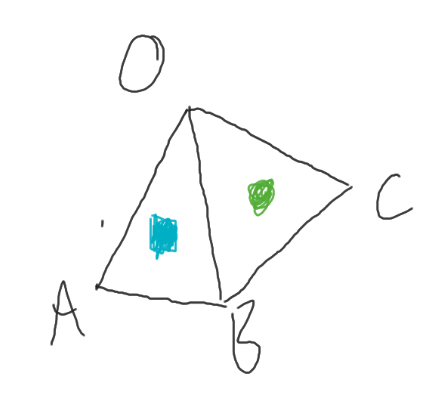
\includegraphics[width=4cm]{tetraedr_1.png}}
\caption{Пирамида OABCD, вид сбоку}
\label{ris:image}
\end{figure}
\begin{figure}[h]
\center{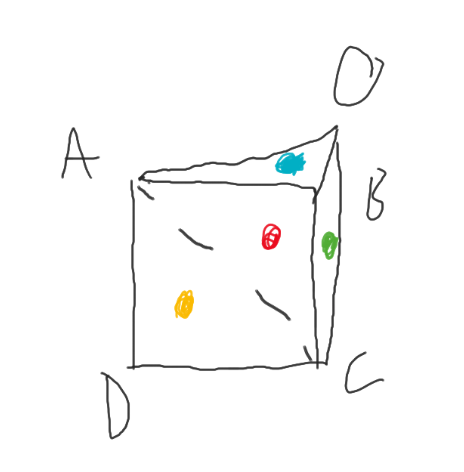
\includegraphics[width=4cm]{tetraedr_2.png}}
\caption{Пирамида OABCD, вид снизу. Нижняя грань разбита на два треугольника}
\label{ris:image}
\end{figure}
\end{center}

\subsubsection{Экран и камера}

Объекты надо как-то отображать на экране. Экран представляется произвольной плоскостью в пространстве, на который проецируются все точки. Поскольку экран имеет ограниченный размер, то и на плоскости выбирается ограниченный прямоугольник. Те точки, которые попадут на прямоугольник экрана, и будут отрисованы. Остальные находятся вне поля зрения.

Для того, чтобы правильно определить, какие объекты видно наблюдателю, используется объект камеры. Этот объект задается своим положением в пространстве ($O_c =  \begin{bmatrix} x_{camera} \\ y_{camera} \\ z_{camera} \end{bmatrix}$), а также матрицей текущего поворота камеры. Назовем ее $M_c$. Еще нам понадобятся габариты параллелипипеда, который видит наша камера~--- координаты ближней левой нижней и правой верхней дальней точки ($(l, b, n)$ и $(r, t, f)$ соответственно).

\subsubsubsection{Шаг 0. Однородные координаты}

Поскольку все операции с координатами имеет смысл выражать через векторы и матрицы, возникает проблема с тем, что не все афинные и проективные преобразования представляются произведением трехмерных матриц. Для этого вводят однородную систему координат, которая работает с четырехмерным пространством по следующему правилу:

$$\begin{pmatrix} x \\ y \\ z \end{pmatrix} \to \begin{pmatrix}x \\ y \\ z \\ 1\\ \end{pmatrix}$$

$$\begin{pmatrix}x \\ y \\ z \\ w\\ \end{pmatrix}, w \neq 0 \to \begin{pmatrix} \frac{x}{w} \\ \frac{y}{w} \\ \frac{z}{w}\end{pmatrix}$$

Такая система разрешает, во-первых, прибавить произвольное число к любой из координат трехмерного вектора:

$$\begin{bmatrix} 1 & 0 & 0 & a_x \\ 0 & 1 & 0 & a_y \\ 0 & 0 & 1 & a_z \\ 0 & 0 & 0 & 1\end{bmatrix} \cdot\begin{bmatrix} x \\ y \\ z \\ 1 \end{bmatrix} = \begin{bmatrix} x + a_x \\ y + a_y \\ z + a_z \\ 1 \end{bmatrix} \to \begin{bmatrix} x + a_x \\ y + a_y \\ z + a_z \end{bmatrix}$$

Также появляется возможноть разделить координаты на произвольную линейную функцию от координат:

$$\begin{bmatrix} 1 & 0 & 0 & 0 \\ 0 & 1 & 0 & 0 \\ 0 & 0 & 1 & 0 \\ k_x & k_y & k_z & 0\end{bmatrix} \cdot\begin{bmatrix} x \\ y \\ z \\ 1 \end{bmatrix} = \begin{bmatrix} x \\ y \\ z \\ k_xx + k_yy + k_zz\end{bmatrix} \to \begin{bmatrix}\frac{x}{k_xx + k_yy + k_zz} \\\frac{y}{k_xx + k_yy + k_zz} \\\frac{z}{k_xx + k_yy + k_zz} \end{bmatrix}$$

Утверждается, что такого дополнительного функционала хватает, чтобы сделать необходимые нам преобразования камеры.

\subsubsubsection{Шаг 1. Сдвиг камеры}
	
Чтобы переместить камеру в центр координат, нужно из каждой координаты $x, y, z$ вычесть ее текущее значение. Это простая единичная матрица с правым столбцом:

$$
\begin{bmatrix}
1 & 0 & 0 & -x(O_c) \\
0 & 1 & 0 & -y(O_c) \\
0 & 0 & 1 & -z(O_c) \\
0 & 0 & 0 & 1
\end{bmatrix}
$$

\begin{center}
\begin{figure}[H]
\center{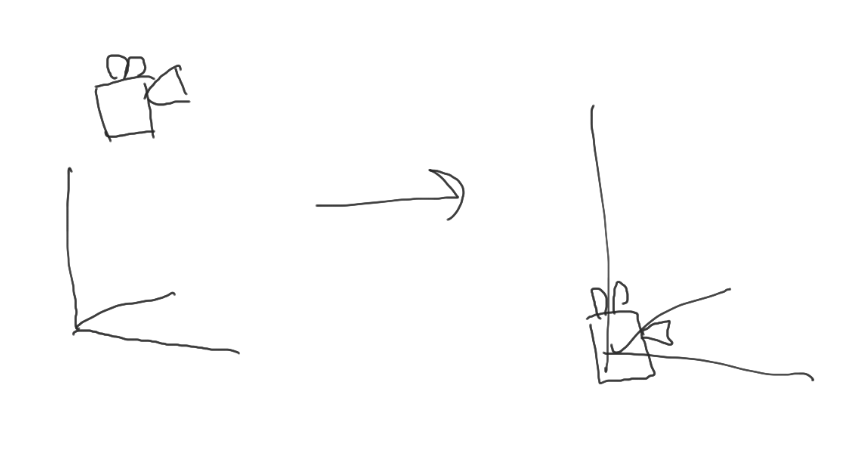
\includegraphics[width=10cm]{step_0.png}}
\caption{Шаг 1. Камера оказывается сдвинута в центр координат.}
\label{ris:image}
\end{figure}
\end{center}

\subsubsubsection{Шаг 2. Поворот камеры}

Для начала стоит понять, как происходит поворот. Если представить себе, что камера задает три ортонормированных вектора, соответствующие осям, то один из векторов остается на месте, а два другие перемещаются, причем в результате преобразований тройка остается ортонормированной. Тогда если мы хотим сделать поворот вокруг оси $oX$, вектор, соответствующий $oX$, остается на месте, в то время, когда оставшиеся два вектора поворачиваются. А именно, происходит преобразование вида $v \to \begin{bmatrix} 1 & 0 & 0 & 0 \\ 0 & \cos \phi & \sin \phi & 0 \\ 0 & -\sin \phi & \cos \phi & 0 \\ 0 & 0 & 0 & 1\end{bmatrix}$, где $\phi$~--- требуемый угол.

\begin{center}
\begin{figure}[H]
\center{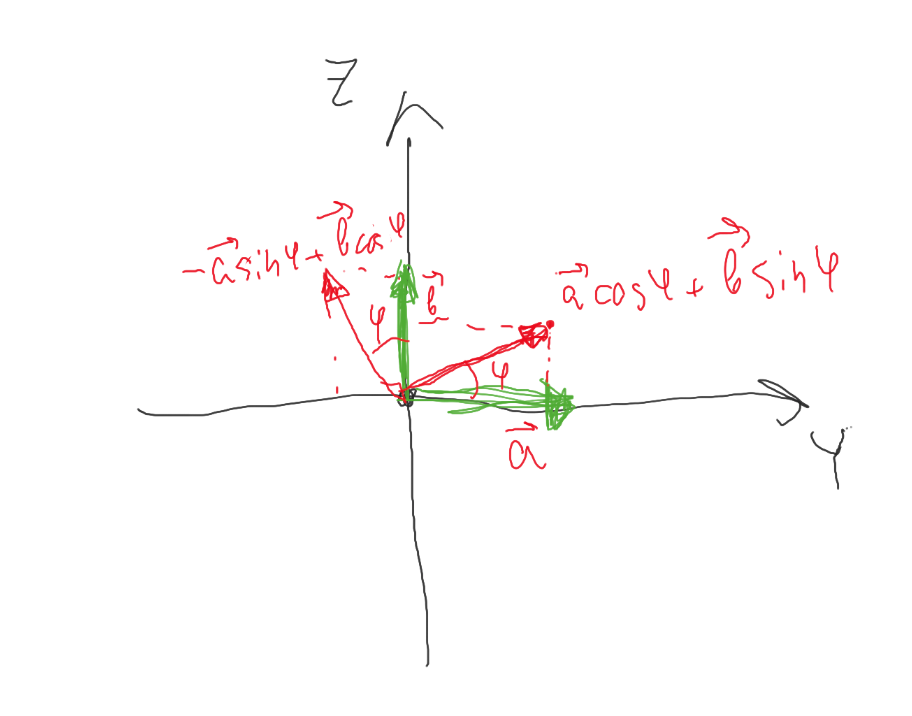
\includegraphics[width=10cm]{rotate_axis.png}}
\caption{Можно видеть, что при повороте базовых векторов в одной плоскости они действительно сдвигаются на один и тот же угол против часовой стрелки}
\label{ris:image}
\end{figure}
\end{center}


Поскольку каждый происходящий поворот камеры является ортогональным преобразованием, то обратное преобразование --- это просто транспонированная матрица всех поворотов. Поскольку мы хотим получить единичную матрицу, то нам надо просто транспонировать матрицу всех преобразований. А именно, если на текущий момент базисные векторы пространства камеры после всех поворотов равны $u, v, w$, то надо сделать такое преобразование:

$$
\begin{bmatrix}
x_u & y_u & z_u & 0 \\
x_v & y_v & z_v & 0 \\
x_w & y_w & z_w & 0 \\
0 & 0 & 0 & 1
\end{bmatrix}
$$

\begin{center}
\begin{figure}[H]
\center{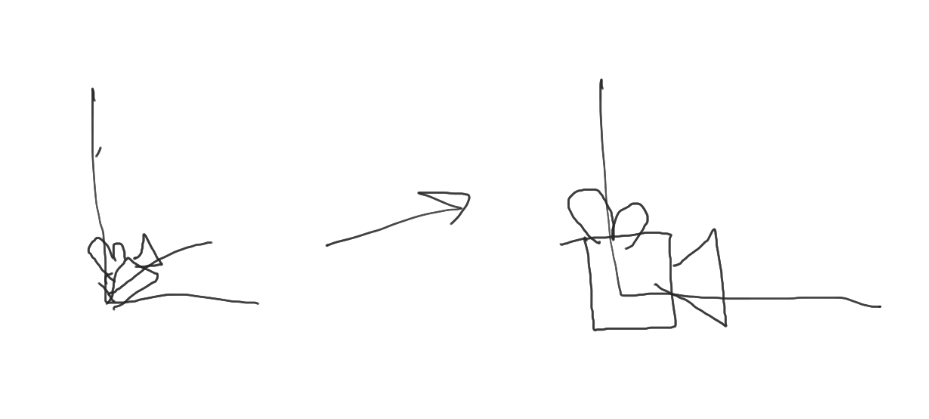
\includegraphics[width=10cm]{step_1.png}}
\caption{Шаг 2. Теперь камера находится в центре координат, плоскость экрана --- декартова система $oXY$, а <<смотрит>> камера в направлении $oZ$}
\label{ris:image}
\end{figure}
\end{center}

\subsubsubsection{Шаг 3. Проективное преобразование}

Для того, чтобы добавить эффект перспективы, область видимости задается в виде усеченной четырехугольной пирамиды. Такой объект сложно спроецировать на экран, поэтому для начала его проективным преобразованием переводят в прямоугольный параллелипипед. После этого проекция оказывается просто отбрасыванием координаты.

У этого подхода есть еще одно приемущество. Отбрасываемая координата задает глубину точки относительно экрана. Поэтому, при прочих равных, надо будет в конкретном пикселе отрисовывать ту точку, которая имела меньшую глубину. Такой метод называется $z$-буфером.

Сначала покажу матрицу, а потом объясню, почему она делает то, что нам  нужно.

$$
\begin{bmatrix}
n & 0 & 0 & 0 \\
0 & n & 0 & 0 \\
0 & 0 & n + f & -nf \\
0 & 0 & 1 & 0
\end{bmatrix}
$$

Матрица проективного преобразвания переведет координаты $(x, y, z, w) \to (nx, ny, (n + f)z - nfw, z) = (\frac{nx}{z}, \frac{ny}{z}, n + f - \frac{- nfw}{z})$. Можно заметить, что первые две координаты домножаются на $\frac{n}{z}$, а от преобразования третьей координаты нам будет важно только то, что оно сохранит знак неравенства. А именно, если раньше у одной точки $z$-координата была больше, чем у другой, то и после преобразования тоже будет больше. Это достигается, потому что от $z$ тут зависит только знаменатель вычитаемого.

А новые двумерные точки (назовем их $x_0$, $y_0$) оказываются верны (с точностью до масштаба) из подобия треугольников, образованных направлением, в котором смотрит камера, и вектором $(x, y, z)$:


\begin{center}
\begin{figure}[H]
\center{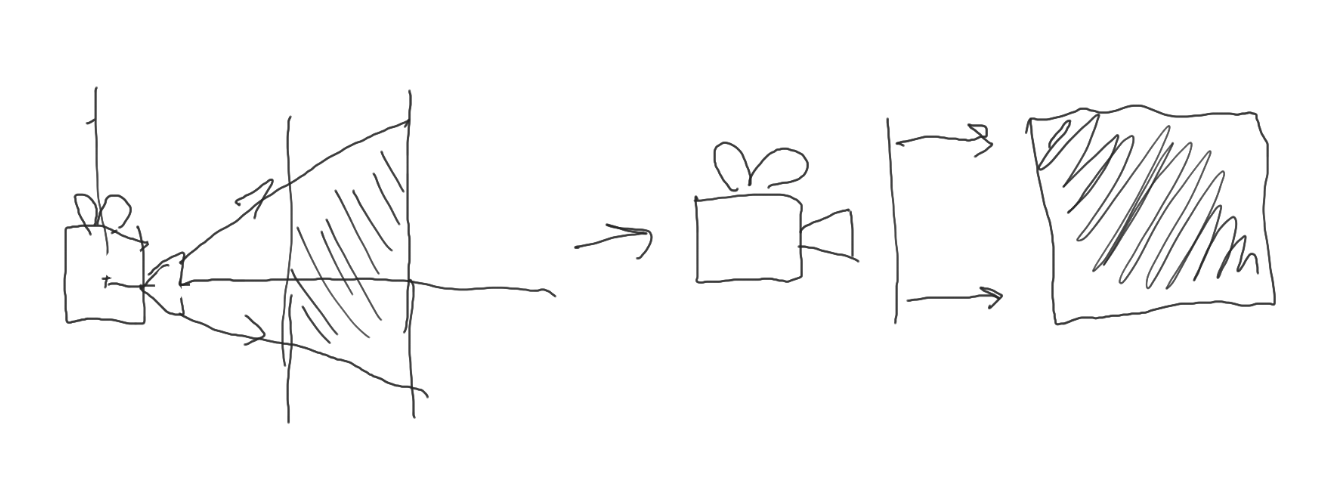
\includegraphics[width=10cm]{step_2.png}}
\caption{Шаг 3. Теперь усеченная пирамида зрения превратилась в параллелипипед зрения}
\label{ris:image}
\end{figure}
\end{center}

\begin{center}
\begin{figure}[H]
\center{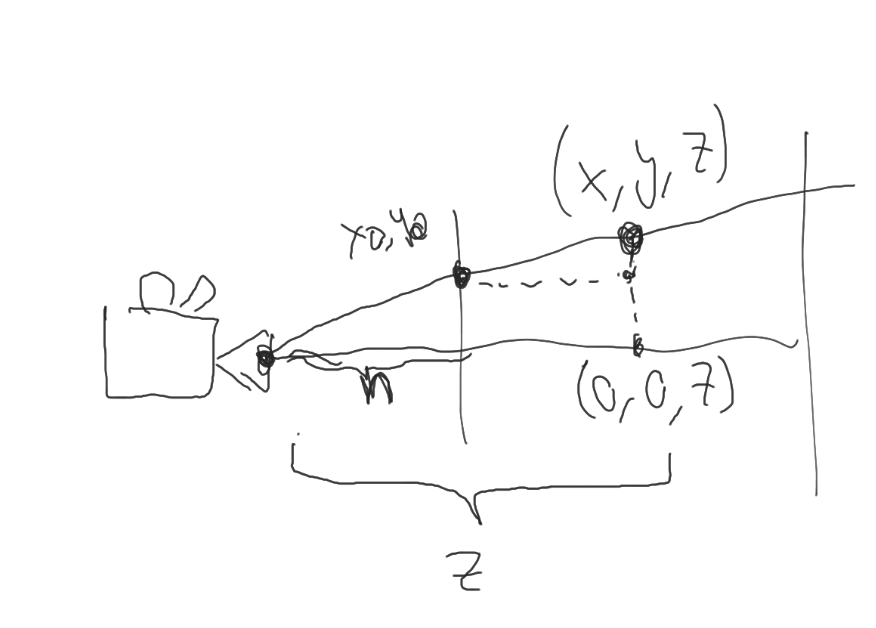
\includegraphics[width=7cm]{z_transform.png}}
\caption{Вот тут можно видеть подобие треугольников}
\label{ris:image}
\end{figure}
\end{center}

\subsubsubsection{Шаг 2,5. Клиппинг}

Можно заметить, что в предыдущем пункте мы делили на $z$. Строго говоря, деление происходило неявно, но, тем не менее, наша операция не обязана быть корректной, если $z$-координата была нулевой. Значит, надо отдельно обработать такой случай.

Чему такой случай соответствует? Тому, что объект находится там же, где и камера. Для нас это означает только одно~--- мы точно его не видим, ведь мы видим только пирамиду обзора, а она находится на каком-то расстоянии от камеры.

Для того, чтобы избавиться от такой проблемы, мы можем просто отфильтровать все объекты, которые оказываются слишком близко к камере. А именно, достаточно выбрать $z_0$~---координату меньше, чем $n$ (потому что при $z$-координате равной $n$, проективное преобразование не сдвигает точку, поэтому она так и окажется на границе), после чего отсечь полупространство с $z$-координатами больше, чем $z_0$. Понятно, что если объект целиком попал по ту или иную сторону полупространства, то выбор бинарный~--- брать объект или не брать. А вот если треугольник пересекает эту плоскость, то задача немного сложнее.

Если у треугольника $ABC$ одна точка (например, $A$) находится в отсекаемой зоне, то требуется найти пересечение отрезков $AB$ и $AC$ с искомой плоскостью (назовем получившиеся точки пересечения $X$ и $Y$). Трапеция $BCYX$ должна быть отображена на экран, это можно сделать с помощью отображения треугольников $BCY$ и $BXY$. Эти треугольники, в свою очередь, не конфликтуют с плоскостью отсечения, поэтому их можно дальше передавать в проективное преобразование и выводить в дальнейшем на экран.

Если у треугольника $ABC$ две точки (например, $AB$) находятся в отсекаемой зоне, то требуется найти пересечение отрезков $AС$ и $BC$ с искомой плоскостью (назовем получившиеся точки пересечения $X$ и $Y$). Треугольник $CYX$ должен быть отображен на экран. Он в свою очередь, не конфликтует с плоскостью отсечения, поэтому его можно дальше передавать в проективное преобразование и выводить в дальнейшем на экран.

Так что клиппинг надо проделать прямо перед проективным преобразованием, после чего перейти к следующим шагам.

\subsubsubsection{Шаг 4. Перемещение параллелипипеда в центр координат}

Чтобы было удобнее дальше работать, параллелипипед перемещается своим центром в центр координат.
$$
\begin{bmatrix}
  1 & 0 & 0 & \frac{-l - r}{2} \\ 
  0 & 1 & 0 & \frac{-b - t}{2} \\
  0 & 0 & 1 & \frac{-n - f}{2} \\
  0 & 0 & 0 & 1\end{bmatrix}
$$


\begin{center}
\begin{figure}[H]
\center{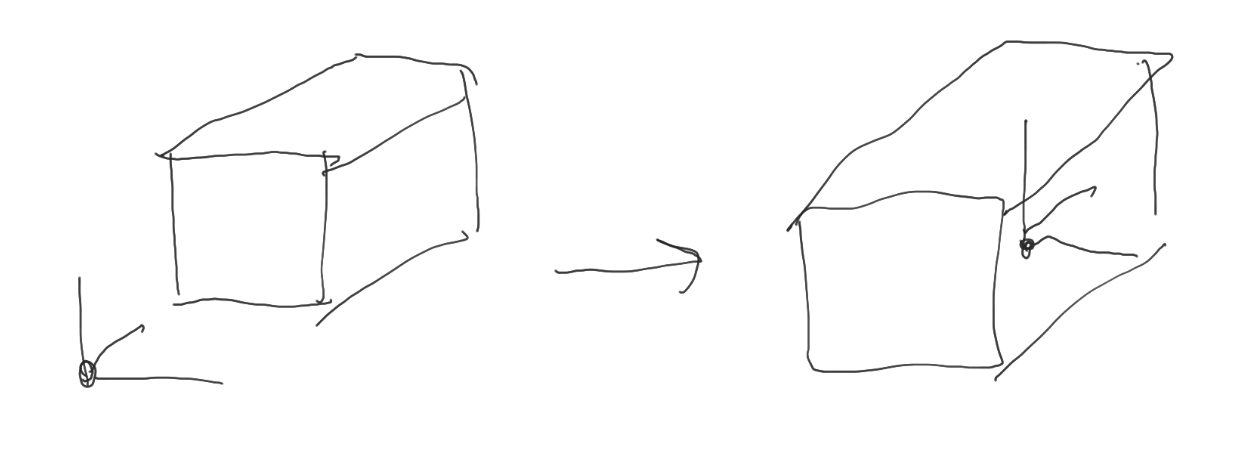
\includegraphics[width=10cm]{step_3.png}}
\caption{Шаг 4. Теперь параллелипипед своим центром оказася в центре координат}
\label{ris:image}
\end{figure}
\end{center}
\subsubsubsection{Шаг 5. Масштабирование в куб $2 \times 2 \times 2$}

Теперь объект масштабируется в куб $(-1, -1, -1), (1, 1, 1)$. Это нужно для того, чтобы в дальнейшем можно было работать с любым экраном.

$$
\begin{bmatrix}
\frac{2}{r - l} & 0 & 0 & 0 \\ 
0 & \frac{2}{t - b} & 0 & 0 \\
0 & 0 & \frac{2}{n - f} & 0 \\
0 & 0 & 0 & 1\end{bmatrix}
$$					  

\begin{center}
\begin{figure}[H]
\center{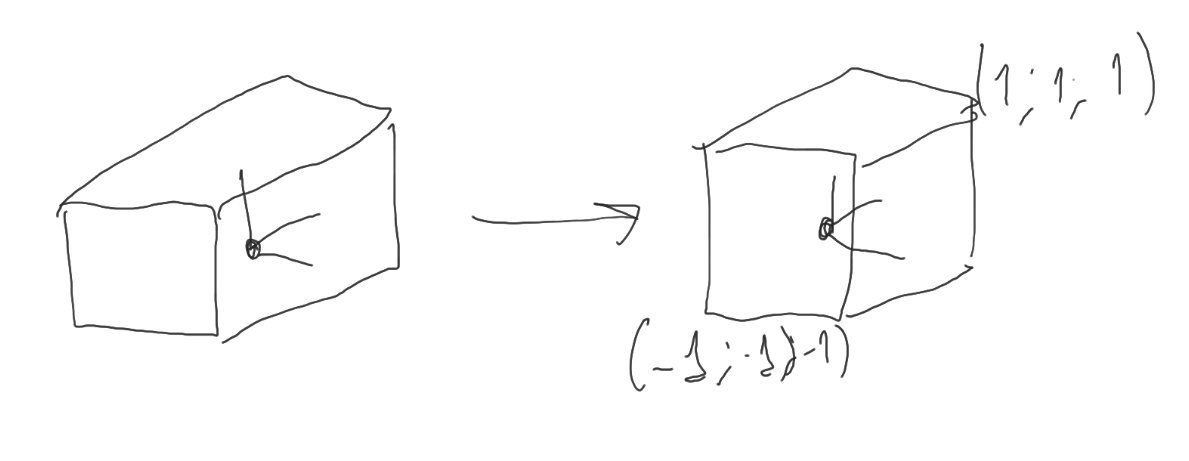
\includegraphics[width=10cm]{step_4.png}}
\caption{Шаг 5. Масштабирование в куб}
\label{ris:image}
\end{figure}
\end{center}

\subsubsubsection{Шаг 6. Перенос в плоскость экрана}

Куб надо отобразить на экране. Для этого мы масштабируем координаты $(x, y)$, а также координата $z$ отвечает за глубину объекта. Можно заметить, что в сдвиге присутствует $\frac{-1}{2}$. Этот сдвиг имеет смысл добавлять, потому что тогда точка перемещается не в угол пикселя, которому она соответствует, а в его центр.

$$
\begin{bmatrix}\frac{Screen_x}{2} & 0 & 0 & \frac{Screen_x - 1}{2} \\ 
0 & \frac{Screen_y}{2} & 0 & \frac{Screen_y - 1}{2} \\
0 & 0 & 1 & 0 \\
0 & 0 & 0 & 1\end{bmatrix}
$$


\begin{center}
\begin{figure}[H]
\center{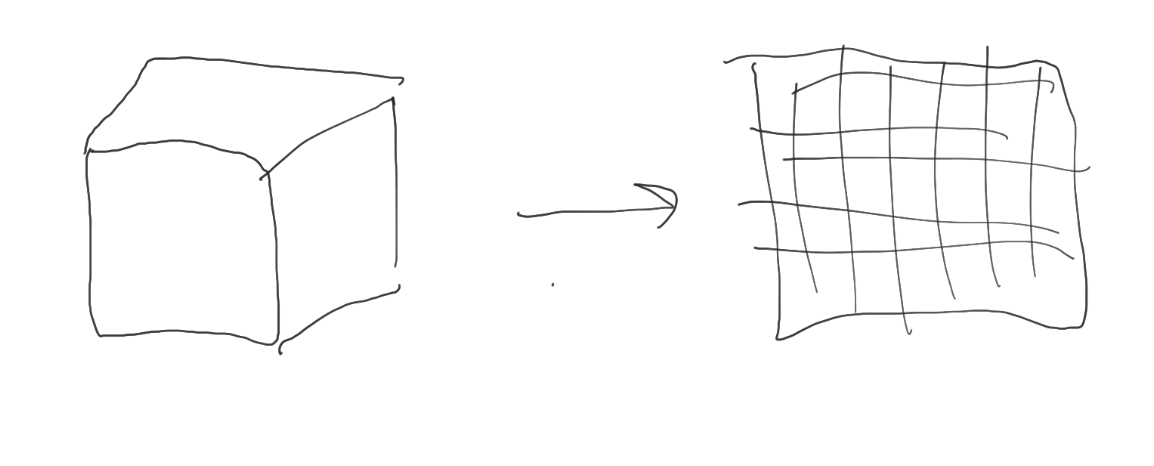
\includegraphics[width=10cm]{step_5.png}}
\caption{Шаг 6. Объект перенесен на экран}
\label{ris:image}
\end{figure}
\end{center}


\subsubsubsection {Здоровенная матрица}
В итоге получается, что камера должна сделать большое преобразование из нескольких матриц:

\begin{enumerate}
	\item Сдвиг камеры в центр координат
	\item Поворот всего мира для перехода в базис камеры
	\item Клиппинг$^*$
	\item Проективное преобразование
	\item Сдвиг центра видимого параллелепипеда в центр координат
	\item Масштабирование в куб $2 \times 2 \times 2$
	\item Прообразование для получения пикселей экрана
\end{enumerate}

$$ M = \begin{bmatrix}\frac{Screen_x}{2} & 0 & 0 & \frac{Screen_x - 1}{2} \\ 
					  0 & \frac{Screen_y}{2} & 0 & \frac{Screen_y - 1}{2} \\
					  0 & 0 & 1 & 0 \\
					  0 & 0 & 0 & 1\end{bmatrix}\begin{bmatrix}
					  \frac{2}{r - l} & 0 & 0 & 0 \\ 
					  0 & \frac{2}{t - b} & 0 & 0 \\
					  0 & 0 & \frac{2}{n - f} & 0 \\
					  0 & 0 & 0 & 1\end{bmatrix}\begin{bmatrix}
					  1 & 0 & 0 & \frac{-l - r}{2} \\ 
					  0 & 1 & 0 & \frac{-b - t}{2} \\
					  0 & 0 & 1 & \frac{-n - f}{2} \\
					  0 & 0 & 0 & 1\end{bmatrix} \cdot $$$$\cdot \begin{bmatrix}
					  n & 0 & 0 & 0 \\
					  0 & n & 0 & 0 \\
					  0 & 0 & n + f & -nf \\
					  0 & 0 & n & 0
					  \end{bmatrix}\begin{bmatrix}
					  x_u & y_u & z_u & 0 \\
					  x_v & y_v & z_v & 0 \\
					  x_w & y_w & z_w & 0 \\
					  0 & 0 & 0 & 1
					  \end{bmatrix}\begin{bmatrix}
					  1 & 0 & 0 & -Camera_x \\
					  0 & 1 & 0 & -Camera_y \\
					  0 & 0 & 1 & -Camera_z \\
					  0 & 0 & 0 & 1
					  \end{bmatrix}$$

Строго говоря, один объект отображается с помощью двух домножений на матрицу. А именно, сначала сделать перенос и поворот, потом сделать клиппинг, после чего сделать оставшиеся шаги.

\begin{center}
\begin{figure}[h]
\center{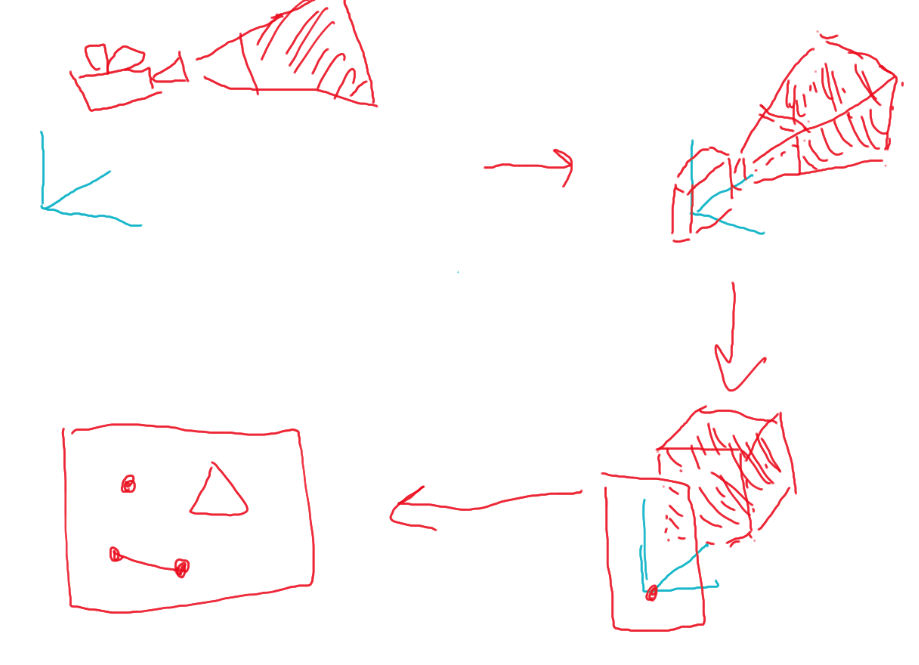
\includegraphics[width=10cm]{camera_pipeline.png}}
\caption{Весь пайплайн отображения объекта}
\label{ris:image}
\end{figure}
\end{center}
\newpage

\subsubsection{Сложность} Для проекции одного треугольника надо сделать не более трех умножений на матрицу $4 \times 4$ (одно до клиппинга и одно или два после), а также $O(1)$ действий на клиппинг, причем клиппинг делает нетривиальные операции только для <<сложных>> объектов~--- тех, для которых надо вычислять координаты пересечения.


\subsection{Отрисовка двумерных объектов}
Дальше происходит отрисовка двумерных объектов на экране по пикселям и заданным вершинам. Для отрезка это достаточно несложная задача, а вот для заливки треугольника нужно придумывать эффективные способы. Автор использует так называемую <<сканирующую прямую>>~--- треугольник отрисовывается послойно, на каждом слое выделяется вертикальная полоса внутри треугольника, и заполняется только она. Вертикальные полосы выбираются только между самой левой x-координатой треугольника и правой x-координатой.

Таким образом, мы сначала перебираем $x$ в отрезке $[min\_x, max\_x]$, затем $y$ в отрезке $[min\_y(x), max\_y(x)]$, после чего $z$ вычисляется как $\frac{(z(x, max\_y) - z(x, min\_y)) \cdot (y - min\_y)}{max\_y - min\_y}$ (это просто линейное масштабирование вектора между крайними точками вертикальной полосы).

Чтобы посчитать $z(x, y)$, нужно выразить точку $(x, y)$ в базисе из двух сторон треугольника, после чего получившиеся коэффициенты применить к исходному четырехмерному треугольнику:

$z(x, y) = z(\alpha \cdot \vec{AB_4} + \beta \cdot \vec{AC_4})$, где $\alpha, \beta$ находятся из уравнения $\begin{bmatrix}\vec{AB_2} & \vec{AC_2} \end{bmatrix} \begin{bmatrix} \alpha \\ \beta \end{bmatrix} = \begin{bmatrix} x \\ y \end{bmatrix}$, а индексы 2 и 4 означают размерность треугольника, в котором берутся векторы.


Осталось понять, как найти min\_y, max\_y.

\begin{center}
\begin{figure}[h]
\center{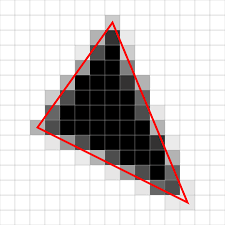
\includegraphics[width=10cm]{triangle.png}}
\caption{Двумерный треугольник. Те клетки, которые пересекаются красной линией, имеют минимальную и максимальную y-координату в своей вертикальной полосе. Клетки между ними и надо закрасить.}
\label{ris:image}
\end{figure}\end{center}


\subsubsection{Сортировка точек в треугольнике}

Прежде, чем заполнять полосу в треугольнике, сделаем предобработку. Для того, чтобы уменьшить число случаев, имеет смысл заранее отсортировать все точки треугольника против часовой стрелки, начиная с самой левой (среди самых левых --- самой нижней). Для этого нужно найти первую точку как самую левую (среди самых левых --- самую нижнюю). Назовем эту точку $A$, а две оставшиеся $B$ и $C$ (их порядок пока что не определен). После чего достаточно вычислить векторное произведение двух векторов $(B - A) \times (C - A)$. Векторное произведение антисимметрично, поэтому мы можем поменять местами точки $B$ и $C$ так, что произведение будет неотрицательным. А это значит, что точка $C$ будет лежать в левой полуплоскости относительно ориентированного отрезка $AB$, что и дает нам отсортированность против часовой стрелки.

\begin{center}
\begin{figure}[H]
\center{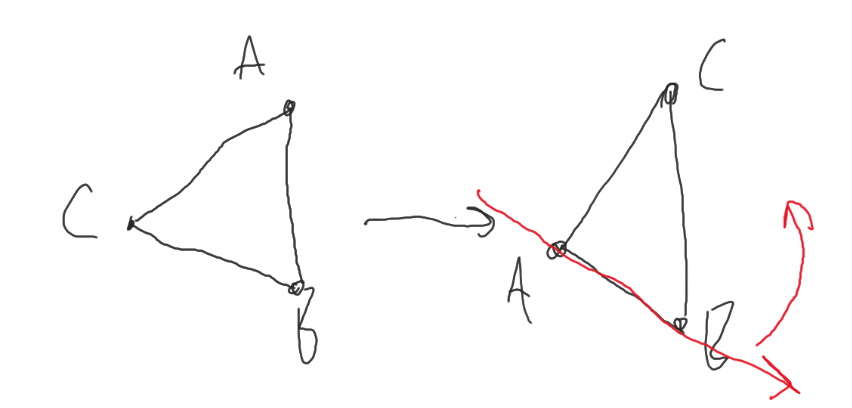
\includegraphics[width=7cm]{sort_triangle_1.png}}
\caption{Треугольник до и после переупорядочивания вершин}
\label{ris:image}
\end{figure}
\begin{figure}[H]
\center{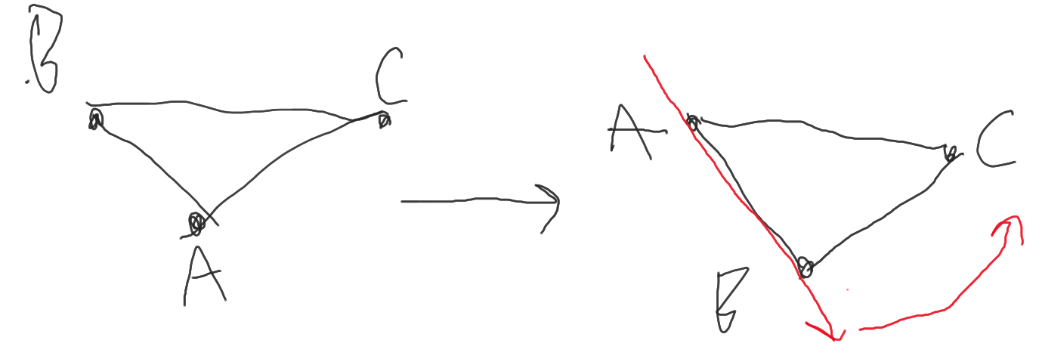
\includegraphics[width=7cm]{sort_triangle_2.png}}
\caption{Еще один треугольник до и после переупорядочивания вершин}
\label{ris:image}
\end{figure}
\end{center}

\subsubsection{Выделение полосы в треугольнике}

На текущей стадии мы хотим для каждой вертикальной полосы в треугольнике найти ее границу. Имеющийся у нас инвариант~--- точки треугольника заранее отсортированы против часовой стрелки, при этом первой в порядке сортировки идет самая левая, а среди самых левых --- самая нижняя.

Теперь для выделения полосы есть всего два случая~--- когда точка $C$ левее точки $B$, и когда правее. В обоих случаях, зная $x$-координату полосы, нужные $y$-координаты вычисляются как точки на соответствующих отрезках. 

Дальше я реализую две симметричные функции для нахождения верхней и нижней границы полосы. Рассмотрим поиск нижней границы. Я смотрю на отрезок $AB$. Если он пересекает полосу, то точка находится на нем, ее можно выразить из линейного уравнения. Если он не пересекает полосу, то точка находится на соседнем отрезке $BC$, линейное уравнение решается для него. Мы добились такого расположения точек за счет предварительной сортировки.


\begin{center}
\begin{figure}[H]
\center{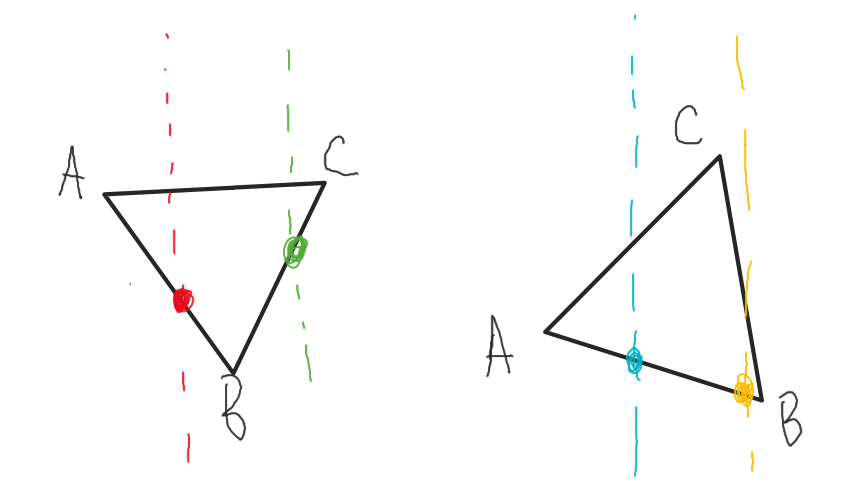
\includegraphics[width=9cm]{sweepline.png}}
\caption{Два случая расположения треугольников. Точки пересечений показывают минимальный $y$ в полосе.}
\label{ris:image}
Соответственно, в зависимости от случая, формулы получаются немного разные, а именно:

Для левой картинки~~$\bigg|$ Для правой картинки

$min\_y(x) = \begin{cases} A.y + \frac{(x - A.x) \cdot (B.y - A.y)}{B.x - A.x} & x < B.x \\ C.y + (\frac{(x - C.x)\cdot (B.y - C.y)}{B.x - C.x} & x \ge B.x\end{cases}$ 
~\bigg|~
$max\_y(x) = \begin{cases} A.y + \frac{(x - A.x) \cdot(C.y - A.y)}{C.x - A.x} & x < C.x \\ B.y + \frac{(x - B.x) \cdot(C.y - B.y)}{C.x - B.x} & x \ge C.x\end{cases}$ 

$max\_y(x) = A.y + \frac{(x - A.x) \cdot(C.y - A.y)}{C.x - A.x}$~\bigg|~$min\_y(x) = A.y + \frac{(x - A.x) \cdot (B.y - A.y)}{B.x - A.x}$
\end{figure}
\end{center}


\subsubsection{Сложность}

Если оценить сложность, то мы выделим необходимую область за $O(w)$, где $w$~--- ширина треугольника. Таким образом, самая неэффективная часть в отрисовке треугольника~--- отрисовка каждого пикселя за $O(S_{\Delta})$. Но поскольку для любого растрового экрана это действие нам понадобится, можно считать, что алгоритм досточно эффективный для нашей задачи.

Таким образом, отрисовка всех объектов происходит за сумму площадей их треугольников.

\newpage

\subsection{Библиотека: описание элементов}

\subsubsection{Авторское: Точки, матрицы, геометрия}

Матрицы Matrix нужны для работы с матричными вычислениями. Пользователю доступно создание матриц произвольного размера, операторы для сложения, вычитания и перемножения матриц. Также доступен поиск обратных матриц, выражение вектора через базис пространства, транспонирование.

Точки Point4d представляют собой набор из четырех координат или матрицу $4 \times 1$. Это объект, который нужен для удобной обертки над несколькими переменными. Для него также доступны арифметические операции, а также отождествление с вектором и возможность нахождения длины. Также есть отождествление 4d-точек с трехмерными через единичную последнюю координату (однородные координаты).

Для работы с двумерной геометрией используется класс двумерного треугольника Triangle2d. Основной его смысл — давать нужную информацию о треугольнике — координаты точек, сохраненные в отсортированном порядке. Также треугольник дает $y$-координаты пересечения вертикальной полосы с собой.

Все многомерные треугольники для отрисовки передаются как объекты класса Triangle4d, который выступает в роли контейнера.

\subsubsection{Авторское: Объекты, мир}

Структура объектов такая: есть объекты типа WireObject, есть объекты типа SurfaceObject, являющиеся наследником типа WireObject. WireObject хранит каркас фигуры: точки и ребра, а SurfaceObject расширяет WireObject данными о триангулированной поверхности объекта. Взаимодействие пользователей происходит с объектами типа SurfaceObject. Мир World является просто контейнером, в котором лежат все объекты. Объекты можно\footnote{ когда-нибудь будет можно, строго говоря} поворачивать и двигать.

И объекты, и мир поддерживают возможность итерирования по своему содержимому: у объектов можно просмотреть все ребра и грани, а у мира можно посмотреть все объекты.

\subsubsection{Авторское: Камера}

Камера Camera отвечает за то, чтобы переводить объекты из системы координат мира в систему координат экрана. Для этого этот объект генерирует матрицу преобразования и применяет ее ко всем точкам, которые надо отобразить. Также камеру можно поворачивать и двигать, что отражается на матрице преобразования.

\subsubsection{Авторское: Экран}

Экран Screen нужен для растрового представления экрана. Он представляет собой несколько табличек с данными по каждому пикселю экрана с возможностью доступа и изменения. А именно, позволяет поставить значение цвета пикселя и узнать текущее значение $z$-буфера в точке.

\subsubsection{Авторское: Renderer}

Renderer отвечает за логику отрисовки. Он принимает набор объектов SurfaceObject, после чего берет отрезки и треугольники в многомерном пространстве, с помощью камеры Camera переносит их в двумерное пространство, выполняет алгоритм растеризации и переносит весь кадр на экран Screen, после чего отрисовывает кадр с помощью библиотеки SFML. 

\subsubsection{Авторское: Application}

Объект Application является основным объектом приложения для пользователя~--- именно оно осуществляет взаимодействие между всеми остальными объектами. Иначе говоря, Application берет все объекты SurfaceObject из контейнера World, после чего просит Renderer отрисовать эти объекты.

Также Application поддерживает интерактивный функционал, доступный в SFML ~--- позволяет пользователю настроить listener-ы на различные системные события, которые умеет отлавливать SFML (например, нажатие на клавиши).

\begin{center}
\begin{figure}[H]
\center{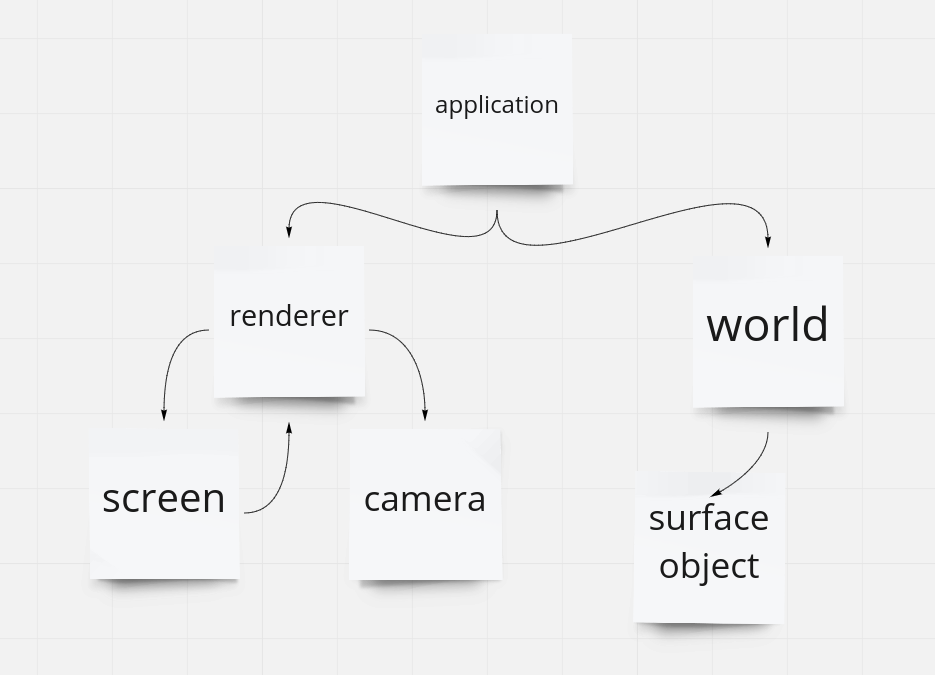
\includegraphics[width=10cm]{class_diagram.png}}
\caption{Взаимоотношение классов. Матрицы, точки и треугольники убраны специально, потому что они используются практически везде, не имеют сложных зависимостей (только треугольники $\to$ точки), а при этом сильно усложнили бы схему. }
\label{ris:image}
\end{figure}
\end{center}

\subsubsection{Стороннее: SFML}

\href{https://www.sfml-dev.org/}{\textcolor{blue}{SFML}} --- это библиотека для отрисовки 2d-графики. У нее есть два основных приемущества:

\begin{enumerate}

\item Достаточно простая.
\item Поддерживает создание интерактивных приложений.

\end{enumerate}

Используется для отрисовки массива точек (растеризованный экран), а также для отрисовки отрезков-ребер.


\newpage
\subsection{Библиотека: Pipeline}

\subsubsection{Описание.}

В итоге Pipeline отрисовки (Application.update(), обновляющий кадр) получился таким:

\begin{itemize}

\item Application.update() вызовет Renderer.prepare(), чтобы очистить экран Screen.clear() и обновить матрицу преобразования Camera.create\_transform()
\item Application.update() вложенными циклами переберет сначала все объекты в мире, а потом все треугольники в объекте.
\item Эти треугольники отправятся на Renderer.draw() --- сначала Camera.project\_point() переведет их в координаты на экране, потом прогоняется алгоритм для двумерного треугольника, который получает пиксели треугольника.
\item Полученные пиксели отправляются в Screen.draw(), который определит ближайший пиксель к плоскости экрана (минимальная z-value)
\item Application.update() в самом конце делает Renderer.update(), который делает Screen.update(), который проходит по всем пикселям и вызывает Renderer.draw() для них, в результате чего множество пикселей оказывается на экране.
\end{itemize}

Отрисовку кадра вызывает пользователь~--- на его усмотрение он может это делать как только после изменений, так и постоянно (например, бесконечным циклом).

\subsubsection{Схема пайплайна.}

\begin{center}
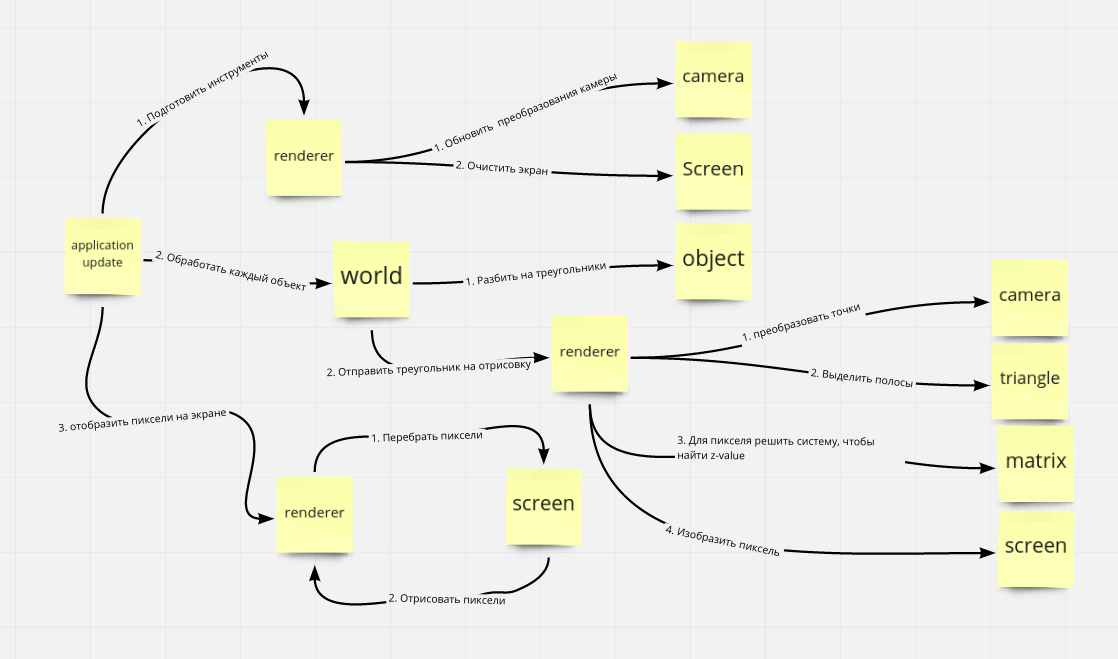
\includegraphics[width=15cm]{scheme_pipeline.png}
\end{center}

\subsubsection{Схема владения объектов}

\begin{center}
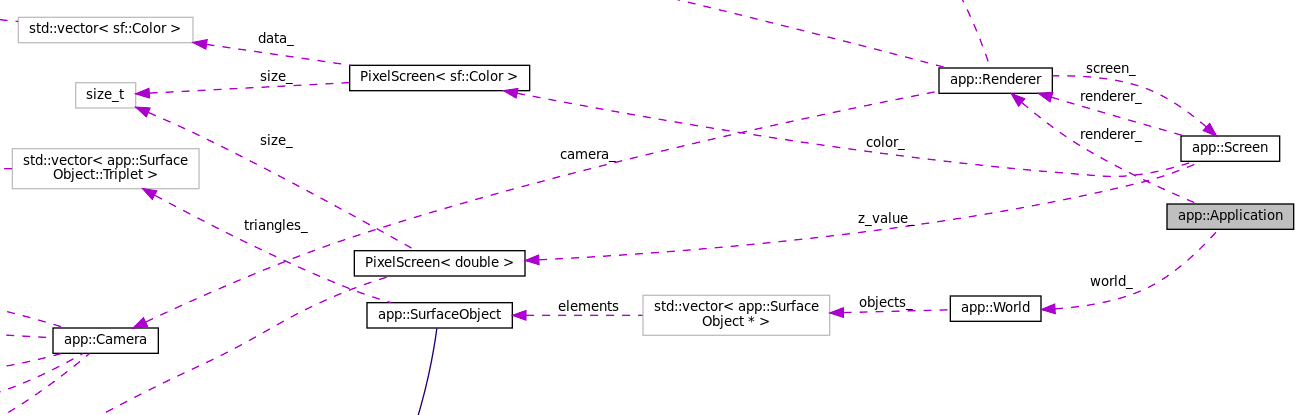
\includegraphics[width=15cm]{scheme_properties.png}
\end{center}

\newpage
\subsection{Тествое приложение и текущие результаты.}

Для теста на текущей стадии разработки используется приложение, в котором можно вращать и двигать кубик. Далее привожу две картинки того, как это у меня выглядит сейчас.

\begin{center}
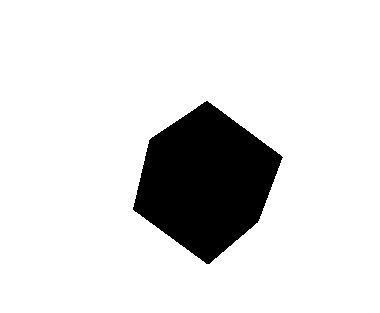
\includegraphics[width=5cm]{cube-1.png}

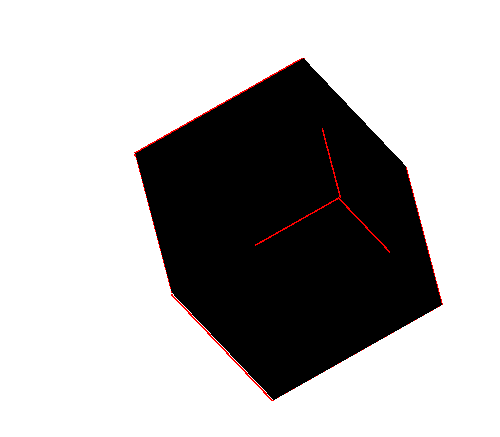
\includegraphics[width=5cm]{cube-2.png}
\end{center}




\bibliographystyle{plainurl}
\bibliography{bibl}

% Здесь текст документа заканчивается
\end{document}
% Начиная с этого момента весь текст LaTeX игнорирует, можете вставлять любую абракадабру.
% 